% Arquivo principal do projeto. Compilar com pdfLaTeX no Overleaf.
\documentclass[a4paper]{article}

\usepackage[utf8]{inputenc}
\usepackage[T1]{fontenc}
\usepackage[brazil]{babel}
\usepackage{graphicx}

\title{Simulador de Escalonamento\\Projeto A: documentação das telas}
% Preencha os autores, se desejar: \author{Nome do aluno \and Nome do colega}
\author{}
\date{}

\begin{document}

\maketitle

\section{Introdução}

Este documento apresenta as telas do simulador de escalonamento do Projeto A,
explica a função de seus elementos visuais e identifica a origem das informações
exibidas. O programa simula tarefas periódicas com os algoritmos preemptivos
Rate Monotonic (RM) e Earliest Deadline First (EDF), utilizando múltiplas CPUs e
um histórico organizado por unidades de tempo, denominadas \textit{ticks}.

A interface é implementada com CustomTkinter. O gráfico de Gantt é desenhado
no Canvas do Tkinter, enquanto a biblioteca drawsvg produz a exportação em SVG.
As figuras são capturas reais da aplicação, reaproveitadas do relatório de telas.
As ampliações correspondem a recortes dessas mesmas capturas.
A lista de eventos do arquivo de configuração pertence ao Projeto B e não é
executada nesta implementação.

O exemplo das figuras de simulação utiliza o arquivo \texttt{configuracao.\allowbreak{}txt},
com RM, duas CPUs e três tarefas periódicas. No repositório de desenvolvimento,
esse arquivo está na pasta \texttt{exemplos}; na versão preparada para envio,
os exemplos estão reunidos na raiz da pasta.

\begin{figure}[htbp]
    \centering
    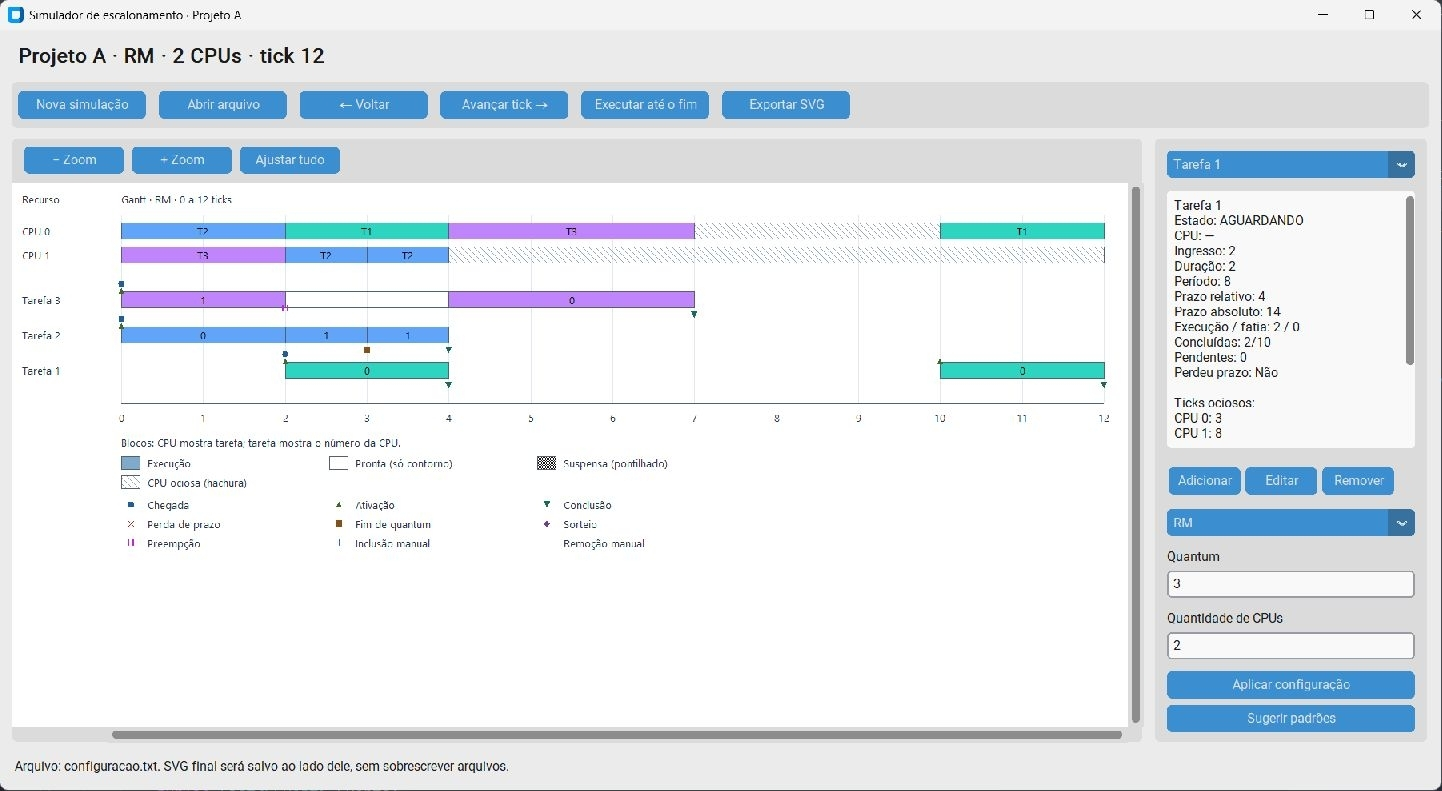
\includegraphics[width=\textwidth]{imagens/principal.png}
    \caption{Janela principal da simulação no tick 12.}
    \label{fig:principal}
\end{figure}

\section{Janela principal}

\subsection{Tela inicial}

A Figura~\ref{fig:inicial} mostra a aplicação antes de carregar ou criar uma
simulação. Nessa situação, o gráfico está vazio e o seletor apresenta a opção
``Sem tarefas''.

\begin{figure}[htbp]
    \centering
    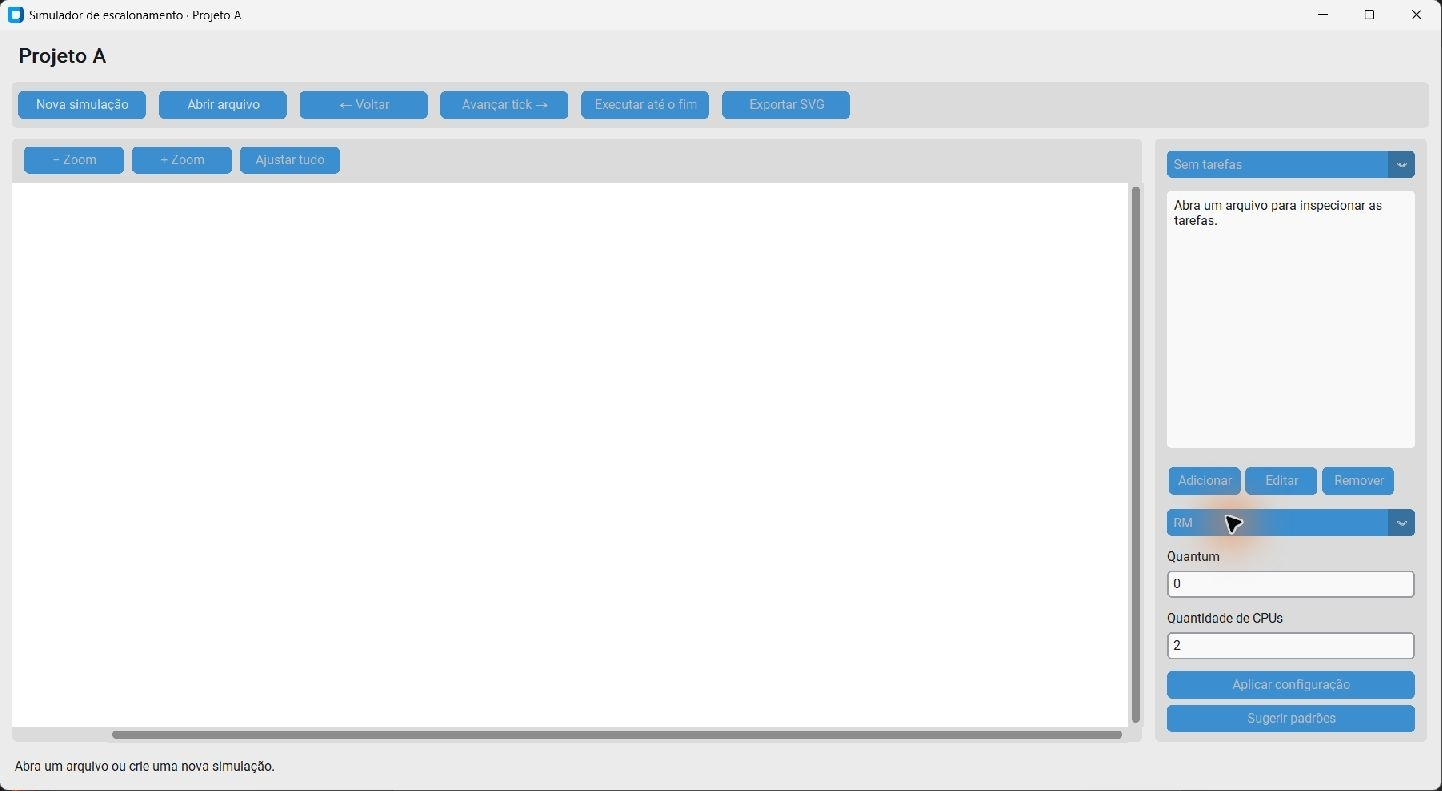
\includegraphics[width=\textwidth]{imagens/inicial.png}
    \caption{Tela inicial, anterior ao carregamento de uma configuração.}
    \label{fig:inicial}
\end{figure}

\begin{description}
    \item[Área do gráfico e seletor.] Permanecem sem dados até que uma simulação
    seja criada ou carregada. O seletor lista as tarefas do estado selecionado.
    \item[Controles disponíveis.] Os botões ``Nova simulação'' e ``Abrir arquivo''
    iniciam o trabalho. Os demais controles dependem da existência de uma simulação.
    \item[Valores iniciais.] As sugestões são quantum 0 e duas CPUs, definidas
    em \texttt{padroes.\allowbreak{}py}. Ainda não há uma simulação em execução.
    \item[Mensagem inferior.] O rodapé orienta o usuário a abrir um arquivo ou
    criar uma nova simulação. O texto é definido pela interface.
\end{description}

\subsection{Navegação e controles}

A Figura~\ref{fig:controles} apresenta a barra de navegação e os controles de zoom.

\begin{figure}[htbp]
    \centering
    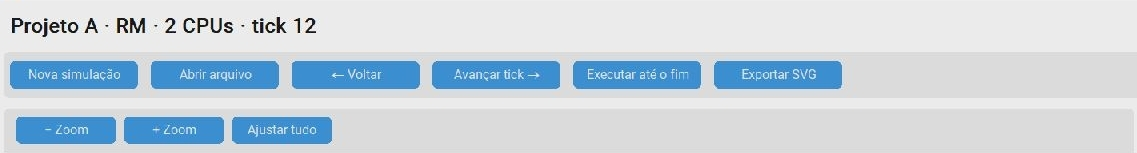
\includegraphics[width=\textwidth]{imagens/controles.png}
    \caption{Resumo da configuração, navegação e controles de visualização.}
    \label{fig:controles}
\end{figure}

\begin{description}
    \item[Título e resumo.] Identificam o Projeto A e mostram algoritmo, quantidade
    de CPUs e tick atual. Os valores vêm de \texttt{Simulacao.\allowbreak{}algoritmo} e
    \texttt{estado\_\allowbreak{}atual}.
    \item[Nova simulação.] Cria um estado vazio no tick 0, com RM, quantum 0 e duas
    CPUs. As sugestões vêm de \texttt{padroes.\allowbreak{}py}; a criação é realizada pelo
    método \texttt{JanelaSimulador.\allowbreak{}nova}.
    \item[Abrir arquivo.] Abre o seletor do Windows. O caminho escolhido é enviado
    a \texttt{parser.\allowbreak{}carregar\_\allowbreak{}configuracao}.
    \item[Voltar e Avançar tick.] Movem o índice do histórico. Avançar reutiliza um
    estado futuro já calculado ou calcula o próximo tick. Voltar não ultrapassa
    o instante zero.
    \item[Executar até o fim.] Avança até que cada tarefa conclua dez ocorrências.
    A interface agenda lotes por \texttt{after()}, e o motor informa o término ou
    eventuais impedimentos, como uma tarefa suspensa.
    \item[Exportar SVG.] Abre a escolha do destino e exporta o histórico até o tick
    selecionado, sem avançar o relógio.
    \item[Menos zoom, Mais zoom e Ajustar tudo.] Alteram somente a escala horizontal
    do Canvas. Ajustar tudo considera o tempo selecionado e a largura disponível.
\end{description}

Os controles são habilitados conforme o estado da aplicação. Durante a execução
em lotes, as intervenções ficam desabilitadas. Após o término, os botões de avanço
e execução completa ficam desabilitados.

\subsection{Gráfico de Gantt}

O gráfico da Figura~\ref{fig:gantt} apresenta duas visões da mesma execução:
as CPUs no topo e as tarefas abaixo. Ambas compartilham o eixo horizontal de tempo.

\begin{figure}[htbp]
    \centering
    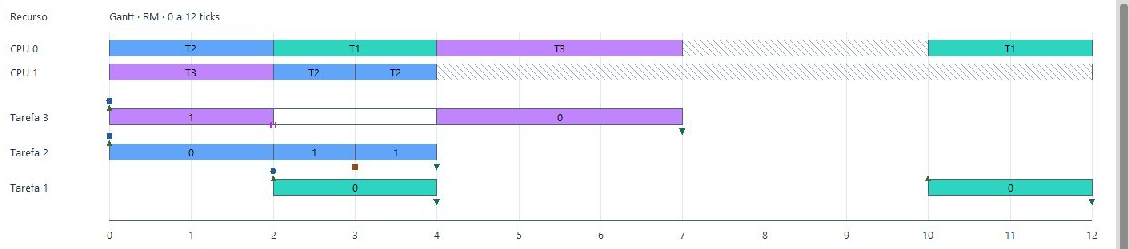
\includegraphics[width=\textwidth]{imagens/gantt.png}
    \caption{Gráfico de Gantt com faixas de CPU e tarefas no tick 12.}
    \label{fig:gantt}
\end{figure}

\begin{description}
    \item[Faixas de CPU.] Mostram qual tarefa executou em cada processador.
    A hachura clara indica que não havia tarefa alocada. A numeração CPU 0,
    CPU 1 e assim por diante corresponde aos identificadores do motor.
    \item[Faixas de tarefas.] São organizadas em ordem decrescente de ID, com a
    tarefa de menor ID mais próxima do eixo do tempo. O número dentro do bloco
    identifica a CPU usada. O texto é branco ou preto conforme a cor de fundo.
    \item[Estado pronta.] É representado por um retângulo apenas com contorno.
    Também é mostrada a espera por CPU logo após a ativação.
    \item[Estado suspensa.] É representado por um preenchimento pontilhado escuro.
    A espera pela próxima ativação periódica permanece sem bloco.
    \item[Eixo do tempo.] Os valores estão em ticks. Um bloco entre $a$ e $b$
    representa o intervalo $[a,b)$.
    \item[Rolagem.] Os rótulos ficam em um Canvas separado: permanecem fixos
    durante a rolagem horizontal e acompanham o gráfico na vertical.
\end{description}

A função \texttt{preparar\_\allowbreak{}gantt} lê o histórico até o instante selecionado.
A função \texttt{coletar\_\allowbreak{}intervalos}, em \texttt{linha\_\allowbreak{}tempo.\allowbreak{}py}, agrupa execução,
espera por CPU, suspensão e ociosidade. A função \texttt{desenhar\_\allowbreak{}gantt} transforma
esses intervalos em coordenadas, tanto no Canvas quanto no SVG.

\subsection{Legenda e eventos}

A Figura~\ref{fig:legenda} mostra os símbolos utilizados no gráfico e na exportação.

\begin{figure}[htbp]
    \centering
    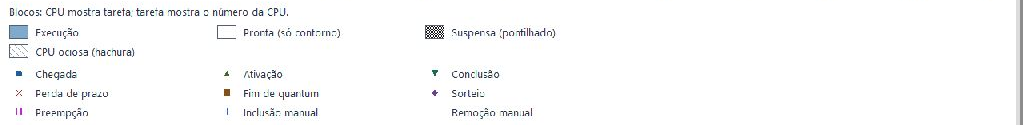
\includegraphics[width=\textwidth]{imagens/legenda.png}
    \caption{Legenda dos estados e eventos do gráfico de Gantt.}
    \label{fig:legenda}
\end{figure}

\begin{description}
    \item[Execução.] A cor vem do TCB no histórico. Na faixa da tarefa, o número
    indica a CPU; na faixa da CPU, o rótulo indica a tarefa. Em trechos muito
    estreitos, é necessário aproximar o zoom para ler os rótulos.
    \item[Contorno, pontilhado e hachura.] Indicam, respectivamente, tarefa pronta,
    tarefa suspensa e CPU ociosa. A espera pela próxima ativação não recebe bloco.
    \item[Chegada.] É indicada pelo polígono circular azul no instante de ingresso.
    Sua origem é o evento \texttt{chegada}, gerado em \texttt{\_\allowbreak{}ativar\_\allowbreak{}tarefas}.
    \item[Ativação.] É indicada pelo triângulo verde para cima. Corresponde ao
    evento \texttt{ativacao}, produzido para uma ocorrência periódica.
    \item[Conclusão.] É indicada pelo triângulo verde para baixo. O evento é
    registrado por \texttt{\_\allowbreak{}concluir\_\allowbreak{}ocorrencia} ao terminar uma ocorrência.
    \item[Perda de prazo.] É indicada por um X vermelho. A origem é a verificação
    realizada por \texttt{\_\allowbreak{}verificar\_\allowbreak{}prazos}. A ocorrência atrasada continua
    executando; concluir exatamente no prazo é válido.
    \item[Fim de quantum.] É indicado pelo quadrado marrom. O término da fatia
    não obriga a tarefa a perder a CPU, caso continue sendo a melhor candidata.
    \item[Sorteio.] É indicado pelo losango roxo nas tarefas escolhidas após o
    desempate por sorteio do escalonador.
    \item[Preempção.] É indicada por duas barras magenta. O evento
    \texttt{preempcao} é registrado em \texttt{\_\allowbreak{}despachar} quando uma tarefa que
    executava deixa de ser selecionada. Migração de CPU e conclusão não geram
    esse evento.
    \item[Inclusão e remoção.] São indicadas pelo sinal de adição e pelo traço,
    respectivamente. O motor registra o instante da intervenção. Os blocos
    passados de uma tarefa removida continuam visíveis no histórico.
\end{description}

O mapeamento de nomes, cores, posições e formas está em \texttt{gantt.\allowbreak{}EVENTOS}
e na função \texttt{marcador}. A interface e o SVG utilizam essas mesmas definições.

\subsection{Seleção e inspeção da tarefa}

A Figura~\ref{fig:inspecao} amplia o painel lateral no tick 12. A barra de rolagem
permite acessar os eventos exibidos abaixo dos contadores.

\begin{figure}[htbp]
    \centering
    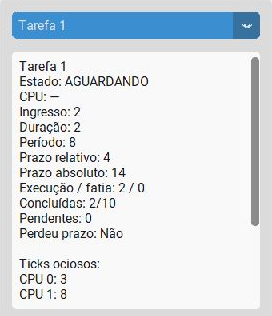
\includegraphics[width=0.65\textwidth]{imagens/inspecao.png}
    \caption{Seletor de tarefa e painel de inspeção.}
    \label{fig:inspecao}
\end{figure}

\begin{description}
    \item[Seletor e identificação.] As opções vêm dos IDs de
    \texttt{estado\_\allowbreak{}atual.\allowbreak{}tarefas}. A opção selecionada determina o TCB inspecionado.
    \item[Estado e CPU.] São obtidos de \texttt{estado\_\allowbreak{}tarefa.\allowbreak{}name} e
    \texttt{id\_\allowbreak{}cpu\_\allowbreak{}atual}. O traço indica ausência de CPU alocada.
    \item[Ingresso, duração e período.] São parâmetros do TCB, provenientes do
    arquivo de configuração, da inclusão ou de uma edição manual aceita.
    \item[Prazo relativo e absoluto.] Correspondem a \texttt{prazo} e
    \texttt{prazo\_\allowbreak{}absoluto}. O prazo absoluto conta da ativação original,
    inclusive quando a ocorrência aguardou na fila.
    \item[Execução e fatia.] Correspondem a \texttt{tempo\_\allowbreak{}exec\_\allowbreak{}instancia} e
    \texttt{tempo\_\allowbreak{}exec\_\allowbreak{}quantum}. Enquanto a tarefa aguarda nova ativação, o
    primeiro contador pode conservar a duração da última ocorrência concluída.
    \item[Concluídas e pendentes.] Mostram \texttt{instancias\_\allowbreak{}concluidas}, de um
    total de dez, e o tamanho de \texttt{ocorrencias\_\allowbreak{}pendentes}. A fila guarda as
    ativações que aguardam a ocorrência anterior terminar.
    \item[Perdeu prazo.] Mostra o indicador \texttt{perdeu\_\allowbreak{}prazo} da ocorrência
    representada pelo TCB, apresentado como SIM ou Não.
    \item[Ticks ociosos.] São os valores de \texttt{tempo\_\allowbreak{}desligada} de cada CPU.
    \item[Eventos do snapshot.] São os dicionários de \texttt{estado\_\allowbreak{}atual.\allowbreak{}eventos}.
    Eles registram o intervalo que produziu o snapshot e as intervenções manuais
    realizadas nesse instante.
\end{description}

\subsection{Configuração do sistema}

A Figura~\ref{fig:configuracao} reúne os controles de tarefas e os parâmetros globais.
Os campos mostram a configuração do snapshot selecionado. A digitação, por si
só, não modifica a simulação.

\begin{figure}[htbp]
    \centering
    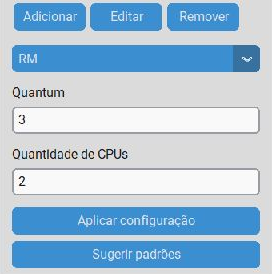
\includegraphics[width=0.65\textwidth]{imagens/configuracao.png}
    \caption{Ações sobre tarefas e configuração global do sistema.}
    \label{fig:configuracao}
\end{figure}

\begin{description}
    \item[Ações sobre tarefas.] Adicionar abre o formulário de inclusão.
    Editar utiliza a tarefa selecionada. Remover retira essa tarefa e sua fila,
    liberando a CPU. As operações são realizadas pelas APIs de \texttt{Simulacao}.
    \item[Algoritmo.] Permite escolher RM ou EDF. O valor inicial vem do arquivo
    ou de \texttt{padroes.\allowbreak{}ALGORITMO}; a política efetiva pertence ao snapshot.
    \item[Quantum.] É um inteiro maior ou igual a zero, obtido de
    \texttt{estado\_\allowbreak{}atual.\allowbreak{}quantum}. Zero remove o limite de fatia, mantendo a
    preempção; valores positivos permitem registrar os fins de fatia.
    \item[Quantidade de CPUs.] É um inteiro maior ou igual a um, obtido do tamanho
    de \texttt{estado\_\allowbreak{}atual.\allowbreak{}cpus}. Reduzir a quantidade libera as tarefas das
    CPUs retiradas.
    \item[Aplicar configuração.] Converte os campos e chama
    \texttt{configurar\_\allowbreak{}sistema}. O motor valida os valores antes de aceitar.
    Uma alteração aceita descarta apenas o futuro do instante selecionado.
    \item[Sugerir padrões.] Preenche RM, quantum 0 e duas CPUs a partir de
    \texttt{padroes.\allowbreak{}py}. O usuário pode substituir as sugestões antes de aplicar.
\end{description}

\section{Formulários de tarefas}

\subsection{Inclusão de tarefa}

A Figura~\ref{fig:inclusao} apresenta o formulário aberto pelo botão Adicionar.

\begin{figure}[htbp]
    \centering
    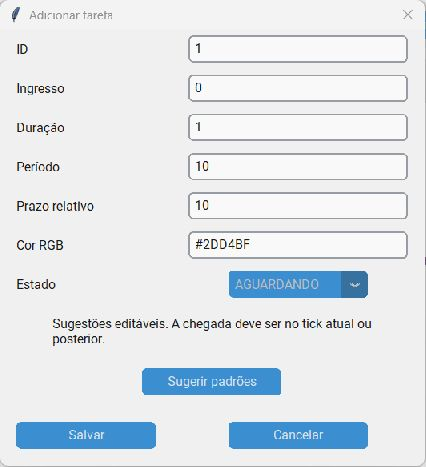
\includegraphics[width=0.65\textwidth]{imagens/inclusao.png}
    \caption{Formulário de inclusão de uma tarefa.}
    \label{fig:inclusao}
\end{figure}

\begin{description}
    \item[ID.] A sugestão é o próximo inteiro positivo disponível no histórico
    selecionado. O campo é editável na inclusão, mas IDs já utilizados nesse
    histórico não podem ser reutilizados.
    \item[Ingresso.] A sugestão é o tick atual. O motor rejeita uma chegada anterior
    ao instante selecionado.
    \item[Duração, período e prazo relativo.] As sugestões são, respectivamente,
    1, 10 e 10 ticks. Os valores devem ser inteiros positivos e podem ser alterados
    antes de salvar.
    \item[Cor RGB.] É sugerida uma cor disponível da paleta. Se necessário, são
    geradas novas cores RGB. O valor deve ter seis dígitos hexadecimais e ser
    distinto das cores das tarefas presentes.
    \item[Estado.] Uma nova tarefa começa em AGUARDANDO. Progresso, CPU, contadores
    e prazo absoluto são inicializados pelo motor.
    \item[Texto de orientação.] Explica que o ingresso deve ocorrer no tick atual
    ou em um instante posterior.
    \item[Sugerir padrões.] Repõe as sugestões produzidas por
    \texttt{Simulacao.\allowbreak{}sugerir\_\allowbreak{}tarefa} e \texttt{padroes.\allowbreak{}py}.
    \item[Salvar.] Envia os campos a \texttt{adicionar\_\allowbreak{}tarefa}. O motor valida a
    operação, e os erros são apresentados no próprio formulário.
    \item[Cancelar e fechar.] Cancelar ou o botão de fechamento da janela encerram
    o formulário sem incluir uma tarefa.
\end{description}

\subsection{Edição de tarefa}

O formulário da Figura~\ref{fig:edicao} recebe os dados do TCB selecionado.
O ID fica bloqueado. Ingresso, duração, período, prazo e cor mantêm os significados
da tela de inclusão. Salvar envia somente os campos alterados ao motor.

\begin{figure}[htbp]
    \centering
    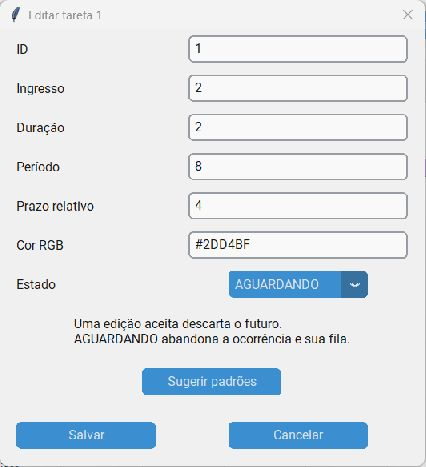
\includegraphics[width=0.65\textwidth]{imagens/edicao.png}
    \caption{Formulário de edição de uma tarefa existente.}
    \label{fig:edicao}
\end{figure}

O seletor de estado permite solicitar as seguintes transições, sujeitas à validação:

\begin{description}
    \item[AGUARDANDO.] Abandona a ocorrência ativa e sua fila, sem acrescentar
    conclusões.
    \item[PRONTA.] Preserva uma ocorrência ativa. Partindo de espera, inicia uma
    ocorrência no tick atual, respeitando o instante de ingresso.
    \item[EXECUTANDO.] Preserva uma ocorrência ativa e exige uma CPU própria ou
    livre. Partindo de espera, também inicia uma ocorrência no instante atual.
    \item[SUSPENSA.] Preserva a ocorrência ativa e seu progresso, liberando a CPU.
    A execução completa exige retomada manual. Partindo de espera, inicia uma
    ocorrência no tick atual, se essa ativação for válida.
    \item[FINALIZADA.] Só é aceita após dez conclusões. Uma tarefa que já concluiu
    dez ocorrências não pode ser reativada.
\end{description}

Na edição, Sugerir padrões preserva ID e estado e sugere parâmetros compatíveis
com o progresso. Cancelar e o fechamento da janela não aplicam mudanças.
A advertência informa que uma edição aceita descarta o futuro. As regras são
implementadas por \texttt{modificar\_\allowbreak{}tarefa\_\allowbreak{}em\_\allowbreak{}execucao} e seus auxiliares.

\section{Mensagens e validação}

As Figuras~\ref{fig:erro-edicao} e~\ref{fig:erro-configuracao} apresentam dois
exemplos de rejeição. Valores inválidos não são aplicados ao estado da simulação.

\begin{figure}[htbp]
    \centering
    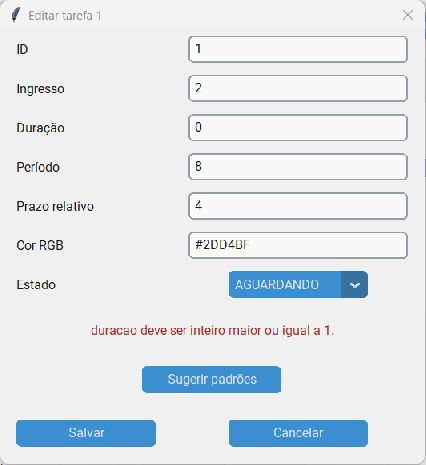
\includegraphics[width=0.60\textwidth]{imagens/erro-edicao.png}
    \caption{Rejeição de uma duração igual a zero no formulário de edição.}
    \label{fig:erro-edicao}
\end{figure}

\begin{figure}[htbp]
    \centering
    
\includegraphics[width=\textwidth]{imagens/erro-configuracao.png}
    \caption{Mensagem no rodapé após informar quantidade de CPUs igual a zero.}
    \label{fig:erro-configuracao}
\end{figure}

\begin{description}
    \item[Mensagem no formulário.] Ao informar duração zero, o motor rejeita o
    valor e a interface apresenta o motivo em vermelho, permitindo a correção.
    \item[Mensagem no rodapé.] Quantidade de CPUs zero é rejeitada. O campo pode
    manter o texto digitado, enquanto o motor conserva a configuração válida
    anterior.
    \item[Arquivo inválido e avisos.] O parser informa o motivo e a linha do erro.
    Campos vazios recebem padrões com aviso; tarefas aperiódicas são ignoradas
    com aviso. Prazo zero é aceito em uma aperiódica ignorada no Projeto A;
    tarefas periódicas exigem prazo positivo.
    \item[Execução e exportação.] Uma tarefa suspensa impede a execução completa,
    e a interface informa o motivo. Falhas de escrita preservam os resultados
    para uma nova tentativa de exportação.
\end{description}

A GUI apresenta erros de valor, execução e entrada ou saída. As exceções
correspondentes são \texttt{ValueError}, \texttt{RuntimeError} e \texttt{OSError}.
As regras básicas estão em \texttt{validacao.\allowbreak{}py}. O motor verifica
as consequências para a ocorrência, a fila e a CPU.

\section{Diálogos de arquivos}

\subsection{Seleção da configuração}

O diálogo Abrir da Figura~\ref{fig:abrir} é fornecido pelo Windows e chamado por
\texttt{tkinter.\allowbreak{}filedialog}. A pasta mostrada na captura é um exemplo de navegação,
não um caminho obrigatório.

\begin{figure}[htbp]
    \centering
    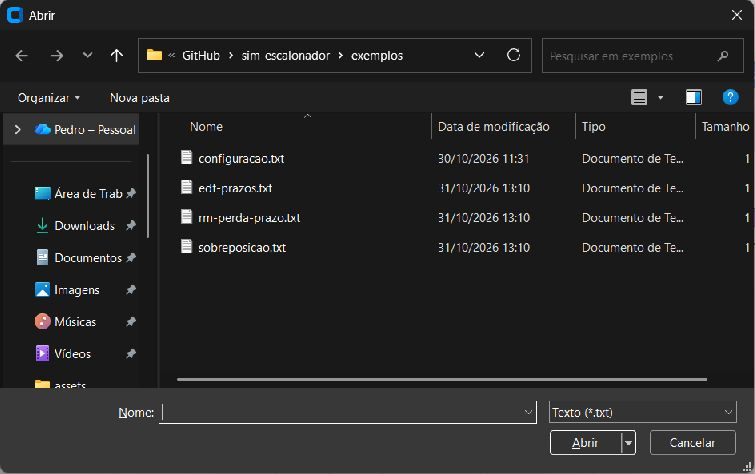
\includegraphics[width=\textwidth]{imagens/abrir.png}
    \caption{Diálogo de seleção de um arquivo de configuração.}
    \label{fig:abrir}
\end{figure}

\begin{description}
    \item[Navegação e endereço.] Mostram a pasta atual, os comandos voltar,
    avançar e subir e os atalhos laterais. São recursos do Windows.
    \item[Busca e ferramentas.] Pesquisar, organizar, criar pasta, alterar o modo
    de exibição e obter ajuda são controles nativos do seletor.
    \item[Lista e colunas.] Nome, data, tipo e tamanho são metadados fornecidos
    pelo sistema de arquivos, não pelo motor da simulação.
    \item[Nome e tipo.] Permitem escolher um nome ou caminho e filtrar os arquivos.
    O filtro inicial é Texto, com extensão \texttt{.\allowbreak{}txt}, e existe a opção Todos.
    As opções são definidas em \texttt{gui.\allowbreak{}abrir}.
    \item[Abrir.] Devolve o caminho ao método \texttt{carregar\_\allowbreak{}arquivo}.
    O parser atua somente depois da escolha.
    \item[Cancelar e fechar.] Encerram o diálogo sem substituir a configuração.
\end{description}

\subsection{Seleção do destino SVG}

O diálogo Salvar como, apresentado na Figura~\ref{fig:exportar}, também é
fornecido pelo Windows. A pasta da captura foi usada apenas para documentar
a operação; o usuário pode selecionar outro destino.

\begin{figure}[htbp]
    \centering
    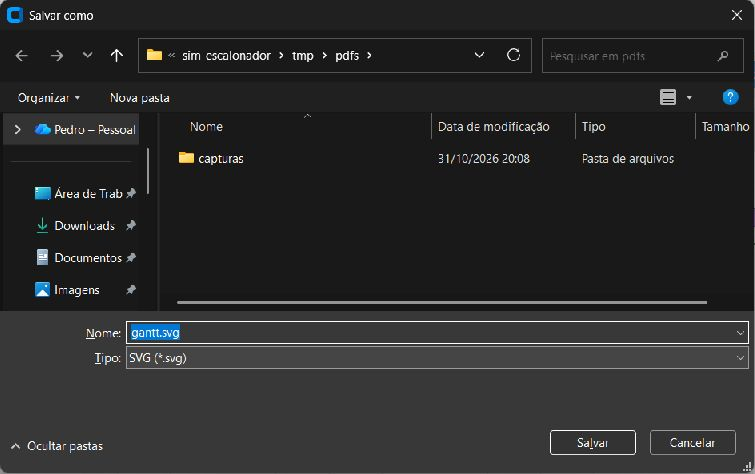
\includegraphics[width=\textwidth]{imagens/exportar.png}
    \caption{Diálogo de seleção do destino da exportação SVG.}
    \label{fig:exportar}
\end{figure}

\begin{description}
    \item[Navegação e lista.] Mostram a pasta de destino e seu conteúdo, fornecidos
    pelo sistema de arquivos. Os atalhos, busca, visualização e criação de pasta
    são recursos do Windows.
    \item[Nome e tipo.] O nome \texttt{gantt.\allowbreak{}svg} é sugerido por
    \texttt{padroes.\allowbreak{}NOME\_\allowbreak{}SVG}. O filtro e a extensão padrão são SVG.
    \item[Salvar.] Devolve o caminho ao método \texttt{exportar\_\allowbreak{}arquivo}.
    O Windows pode solicitar confirmação se o destino já existir.
    \item[Cancelar e fechar.] Encerram o diálogo sem gravar o arquivo.
\end{description}

A função \texttt{gantt.\allowbreak{}exportar\_\allowbreak{}svg} utiliza todo o histórico até o instante
selecionado, com legenda e escala própria. O zoom e a rolagem da interface não
recortam o SVG. Depois da gravação, o rodapé informa o destino. A escolha do
arquivo não altera o estado da simulação nem salva uma configuração.

\section{Resultado final e gravação automática}

O exemplo da Figura~\ref{fig:resultado} termina no tick 185, com dez ocorrências
concluídas para cada uma das três tarefas. O painel mostra a Tarefa 1 como
FINALIZADA e sem CPU. Os campos preservam os dados da última ocorrência, e
o Gantt conserva a execução completa.

\begin{figure}[htbp]
    \centering
    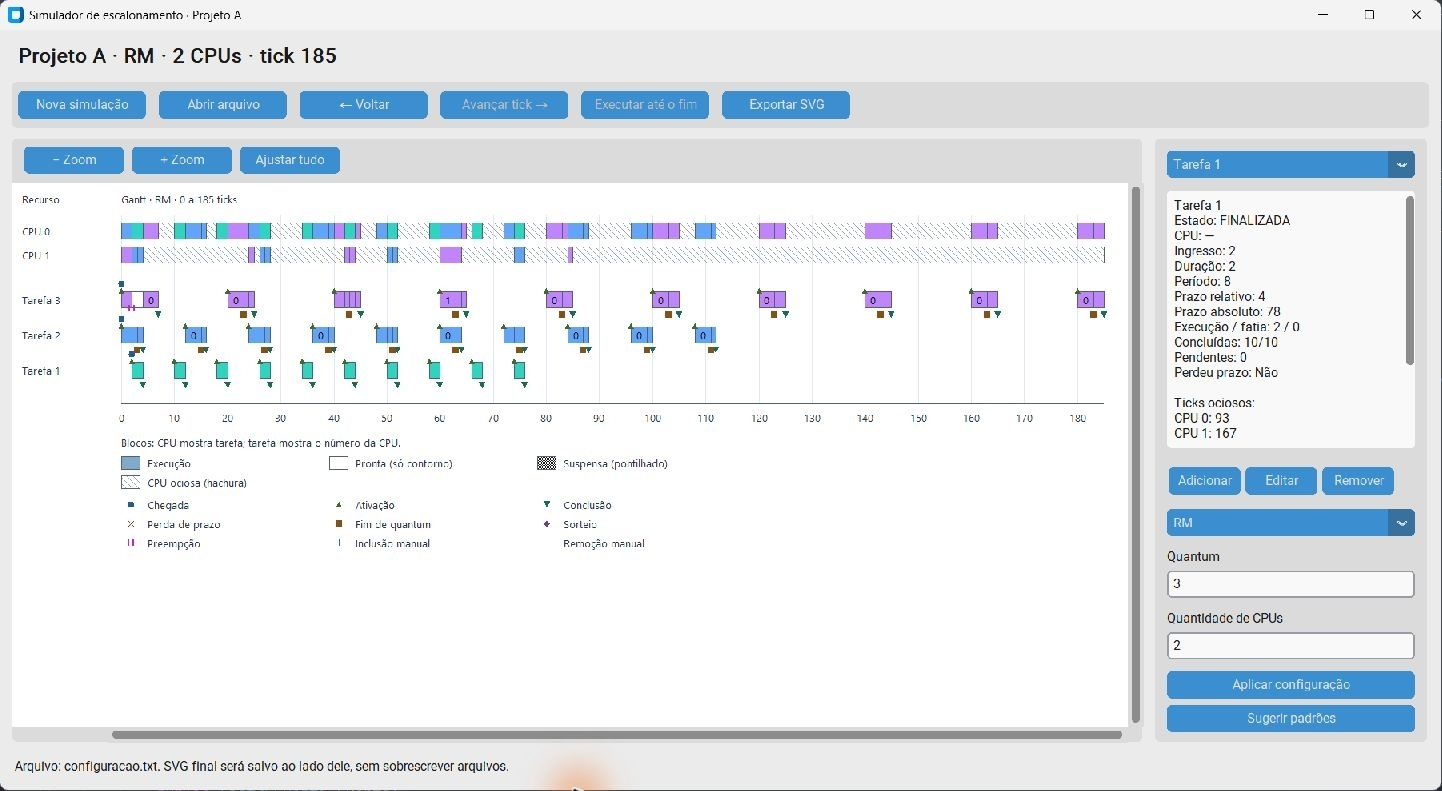
\includegraphics[width=\textwidth]{imagens/resultado.png}
    \caption{Resultado final da configuração de exemplo no tick 185.}
    \label{fig:resultado}
\end{figure}

Ao concluir pela interface com um arquivo de entrada, o método
\texttt{salvar\_\allowbreak{}final} grava um SVG ao lado da configuração. Um sufixo numérico
é acrescentado quando o nome já existe. Sem arquivo de entrada, a interface
solicita um destino. Cancelamento ou falha de escrita preservam o resultado.
O botão Exportar SVG também permite salvar um estado intermediário.

\section{Origem das informações no código}

\begin{description}
    \item[Entrada e sugestões.] \texttt{parser.\allowbreak{}py} converte o cabeçalho e os
    registros de tarefas. \texttt{padroes.\allowbreak{}py} fornece os valores sugeridos.
    \item[Dados do sistema.] As estruturas estão em \texttt{models.\allowbreak{}py}:
    TCB, \texttt{Ocorrencia}, \texttt{Cpu} e \texttt{EstadoSimulacao}.
    A interface consulta o snapshot selecionado pela propriedade
    \texttt{estado\_\allowbreak{}atual} da simulação.
    \item[Evolução e intervenções.] \texttt{engine.\allowbreak{}py} ativa, despacha, executa e
    verifica prazos. Também mantém o histórico e valida configuração, inclusão,
    remoção e edição.
    \item[Prioridades e sorteios.] \texttt{scheduler.\allowbreak{}py} ordena as candidatas por
    RM ou EDF e aplica os desempates. O motor registra os sorteios e as tarefas
    selecionadas nos eventos.
    \item[Intervalos.] O módulo \texttt{linha\_\allowbreak{}tempo.\allowbreak{}py} agrupa
    os trechos do histórico. O módulo \texttt{gantt.\allowbreak{}py} desenha
    intervalos, CPUs e símbolos no Canvas e no SVG produzido por drawsvg.
    \item[Janelas e mensagens.] \texttt{gui.\allowbreak{}py} monta \texttt{JanelaSimulador} e
    \texttt{DialogoTarefa}, lê formulários e apresenta os resultados do motor.
    \texttt{validacao.\allowbreak{}py} valida inteiros, limites, cores RGB e algoritmo.
\end{description}

A configuração usada nas figuras de simulação é:

\begin{verbatim}
RM;3;2
1;2DD4BF;2;2;8;4;
2;60A5FA;0;4;12;8;
3;C084FC;0;5;20;12;
\end{verbatim}

\end{document}
